\chapter{HMC Algorithm for the Schwinger Model}
\label{chap: HMC}

In this chapter we will introduce the case study of this thesis, the Schwinger Model. We previously stated the similarities between this two-dimensional realization of QED and the QCD, hence it will be an efficient toy model for the study of the factorization of the fermionic determinant we want to investigate. Nevertheless, in this first part we should focus on a standard realization of the Schwinger Model on lattice.
\\ Once that we have defined the system we want to simulate, we will give a brief overview of the main properties of the Hybrid Monte Carlo Algorithm, i.e. the algorithm we embed to implement the time evolution of our system. 
\\ Consequently, we will adapt the aforementioned algorithm to our case study, giving all the computational details.
\\ Finally, we will report the results of the tests embedded for the standard Schwinger Model (i.e. with no pre-conditioning), in particular how we gauged the acceptance rate of the HMC algorithm, which must be sufficiently high in the following simulations, where we will actually compute some fermionic observables. 

\section{Schwinger Model}
The Schwinger Model is a two-dimensional realization of QED (QED$_2$), hence a system with $U$(1) gauge symmetry and two mass-degenerate dynamical quarks.
\\ Consider a lattice with $L_0$ thick time slices and spatial extension $L_1$. The space-time points of our lattice $\Lambda$ are labelled by two-integers vectors $n$:
\begin{equation}\label{lattice 2d}
\begin{split}
        \Lambda = \{ n = (n_1, n_2)  | 
        \,\, 0 \leq n_1 \leq L_0 - 1, \,\,\,
        0 \leq n_2 \leq L_1 - 1 \}
\end{split}
\end{equation}
\\ Periodic boundaries conditions (PBC) will be employed in both directions for bosonic degrees of freedom, while fermions will endow PBC along the spatial coordinate and anti-periodic boundary conditions (APBC) in the time direction.
\\ In our lattice formulation we will embed the previously described Wilson-fermions, hence the fermionic part of the action is given by:
\begin{equation}
\begin{split}
    S_F [\psi, \Bar{\psi}, U] &= (m_0 + 2r) \sum_{n, \alpha} \Bar{\psi}_\alpha(n)\psi_\alpha(n) -  \\  
        & - \frac{1}{2}\sum_{\substack{n, \mu \\ \alpha, \beta}}\left[ \Bar{\psi}_\beta(n)(r - \gamma_\mu)_{\beta, \alpha} U_\mu(n) \psi_\alpha(n + \hat{\mu}) + \Bar{\psi}_\beta (n+\hat{\mu}) (r + \gamma_\mu)_{\beta, \alpha} U^\dagger_\mu(n) \psi_\alpha(n) \right] \\
\end{split}
\end{equation}
where $\alpha$ and $\beta$ label the components of the fermionic fields, $m_0$ is the bare mass parameter, we set the Wilson parameter $r = 1$, and $\gamma_\mu$ are the two-dimensional realization of gamma matrices ($\mu = 0, 1$).
In the Dirac basis, $\gamma$-matrices can be written as:
\begin{equation}\label{gammas}
    \gamma_0 = - \sigma_3 = \begin{pmatrix}
 -1 & 0  \\
   0 & 1 \\
\end{pmatrix}
   \,\,\,\,\,\, \gamma_1 = \sigma_1 = \begin{pmatrix}
 0 & 1  \\
   1 & 0 \\
\end{pmatrix}
   \,\,\,\,\,\, \gamma_2 = i\gamma_0 \gamma_1 = \sigma_2 = \begin{pmatrix}
 0 & -i  \\
   i & 0 \\
\end{pmatrix}
\end{equation}
where $\sigma_i$ ($i = 1, 2, 3$) are the Pauli matrices. Analogously to what we have seen before, we can define the Dirac-Wilson operator acting on two quarks defined in $m$ and $n$ as:
\begin{equation}\label{D}
\begin{split}
        D_{\beta, \alpha} (m, n) = &(m_0 + 2) \delta_{\beta, \alpha} \delta_{m,n} - \\ &- \frac{1}{2}\sum_{\mu} \left[ (1 - \gamma_\mu)_{\beta, \alpha} U_\mu(m) \delta_{n, m+\hat{\mu}} + (1 + \gamma_\mu) U_\mu^\dagger (m - \mu)_{\beta, \alpha} \delta_{n, m - \hat{\mu}} \right]
\end{split}
\end{equation}
This operator satisfies the so called $\gamma_2$-hermiticity, hence:
\begin{equation}
    D^\dagger = \gamma_2 D \gamma_2
\end{equation}
and the Hermite-conjugate of the Dirac operator can be written as:
\begin{equation}\label{D daga}
\begin{split}
         D^\dagger_{\beta, \alpha} (m, n) & = (m_0 + 2) \delta_{\beta, \alpha} \delta_{m,n} - \\ 
         & - \frac{1}{2}\sum_{\mu} \left[ (1 - \gamma_\mu)_{\beta, \alpha} U_\mu^\dagger(m - \mu) \delta_{n, m - \hat{\mu}} + (1 + \gamma_\mu)_{\beta, \alpha} U_\mu (m) \delta_{n, m + \hat{\mu}} \right]
\end{split}
\end{equation}
Finally, the fermionic action can be rewritten as:
\begin{equation}
\begin{split}
    S_F[\psi, \Bar{\psi}, U] & = \sum_{\substack{n, m \\ \alpha, \beta}} \Bar{\psi}_\beta(m) D_{\beta, \alpha}(m, n) \psi_\alpha(n) = \\
    & = \sum_{n, \alpha} \Bar{\psi}_\alpha(n) \psi_\alpha(n) - \kappa \sum_{n, \mu} \left[ \Bar{\psi}(n)(1 - \gamma_\mu) U_\mu(n) \psi(n+\hat{\mu}) + \right. \\ & \hspace{40mm} \left. + \Bar{\psi}(n)(1 + \gamma_\mu) U_\mu^\dagger (n - \mu) \psi(m - \hat{\mu}) \right]
\end{split}
\end{equation}
where $\kappa = \frac{1}{2(m_0 + 2)}$.
For what concerns the gauge part, the action is given by:
\begin{equation}\label{Sg}
        S_G[U] = -\beta \sum_{P} \Re{U_P}
\end{equation}
where
\begin{equation*}
    U_P(n) = U_\mu(n) U_\nu (n + \hat{\mu}) U^\dagger_\mu(n+\hat{\nu}) U^\dagger_\nu(n) = U_0(n) U_1 (n + \hat{0}) U^\dagger_0(n+\hat{1}) U^\dagger_1(n)
\end{equation*}
is the standard plaquette in (1+1) dimensions. Recall that $U_\mu(n) \in U(1)$ is a link-variable connecting points $n$ and $n + \hat{\mu}$ of the lattice, with $\mu = 0, 1$.
Accordingly to the current state of art of computatational techniques for lattice gauge theories, in order to simulate our system we first require to integrate out analytically the fermionic degrees of freedom. Since we are working with two mass-degenerate quark flavors, the partition function is given by:
\begin{equation*}
    Z = \int \mathcal{D}[U]\, e^{-S_G[U]} \det[D] \det[D]
\end{equation*}
We can recast this expression in order to obtain an effective gauge theory which can be simulated through Monte Carlo algorithms, where we exploit gauge configuration properly distributed according to the gauge action. Nevertheless, this process comes with downsides, as the locality of the original action is not manifest anymore, as the fermion determinant is a non-local functional of the links $U$. 
\\ In our simulations, accordingly to the previous expression, we can interpret the fermion determinant as a probability weight factor when generating gauge configurations, since it is real (thanks to $\gamma_2$-hermiticity) and non-negative. Hence we will define a Monte Carlo algorithm which draws gauge configurations with the following probability distribution:
\begin{equation*}
    \frac{1}{Z}\,e^{-S_G[U]} \det[D] \det[D] =  \frac{1}{Z}\,e^{-S_G[U]} \det[D D^\dagger]
\end{equation*}
To introduce a bosonic effective action, we can express $\det[DD^\dagger]$ as the result of a bosonic Gaussian integral over $N$ complex variables $\phi$:
\begin{equation}
    \det[DD^\dagger] =  \pi^{-N} \int \mathcal{D}[\phi_R] \mathcal{D}[\phi_I] \, e^{-\phi^\dagger (DD^\dagger)^{-1} \phi}
\end{equation}
and we refer to $\phi$ as pseudofermion fields, i.e. bosons with the same number of degrees of freedom as fermions. If the number of mass-degenerate fermions is even, we can guarantee positivity, hence the convergence of the Gaussian integral.
\\ Then we can define the \textit{effective fermion action}:
\begin{equation}
    S_F^{\textrm{eff}} [U] = \phi^\dagger (DD^\dagger)^{-1} \phi
\end{equation}
which is highly non-local, as it basically connects all the link variables of the lattice with each other.
In conclusion, a possible way to include dynamical fermions in our simulations consists in generating gauge configurations in our Markov Chain accordingly to the Boltzmann weight factor:
\begin{equation}
    \exp(-S[U]) \hspace{10mm} \mbox{with:} \hspace{2mm} S[U] = S_G[U] + S_F^{\textrm{eff}} [U]
\end{equation}
In the next chapter we introduce the algorithm typically used (within its variants) for the simulation of lattice gauge theories, the Hybrid Monte Carlo (HMC) algorithm \cite{DUANE1987216}.  

\section{Hybrid Monte Carlo}
This algorithm is based on the concept of Markov Chains, hence a sequence of configurations-drawings which represent the dynamical evolution of our system in the computer time (or \textit{Markov time}, $\tau$), accordingly to the desired probability distribution $\exp(-S[U])$.
\\ The name \textit{hybrid} comes from the fact that the candidates for the new gauge-configurations come from the evolution of classical Molecular Dynamics (MD) equations of motion, and the algorithm is completed by a following step where the proposal gets accepted or rejected as in the Metropolis-Hastings algorithm. Let us see these two steps more in detail.
\\ The overall transition probability from one configuration to the following one is given by two terms. Starting from a gauge configuration $U$, through the MD leapfrog evolution scheme we will propose a new candidate $U'$, introducing an a priori selection probability factor $T_0(U' | U)$. Nextly, we decide whether to accept the proposal accordingly to the acceptance probability:
\begin{equation}
    T_A (U'|U) = \min \left(1, \frac{T_0(U|U') e^{-S[U']}}{T_0(U'|U) e^{-S[U]}}\right)
\end{equation} 
Putting all together, the overall transition probability is:
\begin{equation*}
    T(U'|U) = T_A(U'|U)T_0(U'|U)
\end{equation*}
Since we are interested in ergodic Markov Chains, we require this probability to obey the detailed balance condition:
\begin{equation}
    T(U'|U) P(U) = T(U|U')P(U')
\end{equation}
hence the probability of drawing the configuration $U$ and transitioning from $U \to U'$ must be equal to the probability of drawing $U'$ and then evolve $U' \to U.$ An explicit proof of the fact that the HMC algorithm satisfies the detailed balance condition can be found in Appendix \ref{app:a}.
\subsection{HMC Algorithm for the Schwinger Model}
Here we will show more in-depth the steps of the algorithm for our case study.
\\ Consider the system described previously, with the introduction of pseudofermion fields $\phi$. We want to draw configurations distributed accordingly to the Boltzmann weight factor:
\begin{equation}
    \exp(-S[U]) = \exp(\beta \sum_P \Re{U_P} - \phi^\dagger (DD^\dagger)^{-1}\phi )
\end{equation}
and in our evolution scheme, pseudofermion fields and gauge fields will be updated alternatively. The dynamical evolution of this system is given by the following steps.
\begin{itemize}
    \item \textbf{Step 1 (Pseudofermions):} We want to generate pseudofermion fields according to the Gaussian distribution $e^{- \phi^\dagger (D D^\dagger )^{-1} \phi}$. To achieve this, we can generate a complex vector $\chi$ according to a Gaussian distribution $e^{-\chi^\dagger\chi}$, and then compute $\phi = D\chi$.
    \\ Pseudofermion fields will be kept fixed during the time evolution of the gauge fields.
    \item \textbf{Step 2 (Conjugate variables)}: We will consider as conjugate variables the gauge fields $U_\mu(n)$ and a set of momenta $\pi_{\mu}(n)$ distributed according to a Gaussian $e^{-\Pi^2/2}$. Notice that $U_\mu(n)$ is a $U(1)$ group element, i.e. a phase factor, and it can be written as: 
    \begin{equation*}
        U_\mu(n) = \exp(iQ_\mu(n)) \,\,\,\,\mbox{with }\,\, n \in \Lambda, \, \mu = 0,1  \,\,\mbox{and}\,\,\,Q_\mu \,\,\mbox{real}
    \end{equation*}
    \item \textbf{Step 3 (Leapfrog equations):} The classical set of equations of motions for conjugate variables $Q$ and $\pi$ such that $H[Q, \pi] = \frac{1}{2} \pi^2 + S[Q]$ is:
    \begin{equation}\label{EOM}
    \begin{split}
        \dot{Q} &= \pdv{H}{\pi} = \pi \\
        \dot{\pi} &= -\pdv{H}{Q} = - \pdv{S}{Q}
    \end{split}
    \end{equation}
    where the derivatives understand a derivation with respect to a field value at a single lattice site.
    \\ These equations of motion are derived by asking $\Dot{H} = 0$, hence that the Hamiltonian is a constant of motion. If we could implement the dynamical evolution exactly, the proposals for the gauge configurations would always be accepted, but this is not the case, since the evolution scheme will be integrated numerically. 
   \\ Nevertheless, by following the so-called leapfrog integration scheme, we can derive a dynamical evolution which satisfies the detailed balanced condition, since the MD trajectory is reversible.\footnote{Reversibility is given by the condition: $T(Q', \pi'|Q, P) = T (Q, -\pi|Q', -\pi')$. In order to satisfy the detailed balance condition, the MD trajectory must also guarantee the area preservation of the integration measure $\mathcal{D}[\pi]\mathcal{D}[Q]$.}.
    \\ To integrate the classical equations of motion, we will implement a numerical integral with a discrete step size $\varepsilon = \Delta \tau$. 
    \\ The real phases $Q$ are evolved in $n$ steps of length $\varepsilon$, while the conjugate momenta $\pi$ start with a half-step $\varepsilon/2$, then they undergo $(n-1)$ full steps and finally again a half-step. Iterating this steps we build a molecular dynamics trajectory: we can combine $n$ leapfrog steps to build a trajectory of length $n \varepsilon \simeq 1$. 
    \\ Since we are integrating these equations numerically, the evolution scheme is only approximately correct, as numerical errors must be taken into account: the discretization error for half-steps is $\mathcal{O}(\varepsilon^2)$, for full steps it is $\mathcal{O}(\varepsilon^3)$. 
    \\ In the next subsection we will compute the integration scheme explicitly.
    \item \textbf{Step 4 (Accept/Reject)}: Once that the final step of the trajectory is reached, we accept the proposal $(Q(\tau), \pi(\tau)) \to (Q(\tau + n\varepsilon), \pi(\tau + n \varepsilon)) \equiv (Q', \pi')$ if:
    \begin{equation*}
        r < \frac{\exp{-H[Q(\tau + n\varepsilon), \pi(\tau + n\varepsilon)]}}{\exp{-H[Q(\tau), \pi(\tau)]}}
    \end{equation*}
    where $r$ is a random number in $[0,1).$
\end{itemize}
\subsection{Leapfrog evolution scheme}
In the previous section we have seen the molecular dynamics equations (\ref{EOM}), now we want to solve them explicitly for our system. To keep track of the evolution in the computer time $\tau$, we add an extra label $k = 0, \dots, n$ that denotes the particular evolution step at which we evaluate the variables. For the sake of clarity, $x \in \Lambda$ will now refer to space-time points of the lattice.
\\ \textbf{First step:} We start with a half-step for the evolution of the conjugate momenta $\pi$, and from (\ref{EOM}):
\begin{equation}\label{first step pi}
    \pi_{\mu,0}(x) \to \pi_{\mu, \frac{1}{2}}(x) =  \pi_{\mu,0}(x) - \left. \pdv{S}{Q_\mu(x)} \right\rvert_{Q_{\mu, 0}} \frac{\varepsilon}{2}
\end{equation}
We need to evaluate the derivative of the action $S[U] = S_G[U] + \phi^\dagger (D D^\dagger )^{-1} \phi$ with respect to $Q_\mu$. For what concerns the gauge action, recall that:
\begin{equation*}
\begin{split}
    \Re{U_P} & = \frac{1}{2}(U_P + U_P^\dagger) = \\
             & = \frac{1}{2} \left[  U_\mu(n) U_\nu (n + \hat{\mu}) U^\dagger_\mu(n+\hat{\nu}) U^\dagger_\nu(n) + U_\nu(n) U_\mu (n + \hat{\nu}) U^\dagger_\nu(n+\hat{\mu}) U^\dagger_\mu(n) \right] \\
\end{split}
\end{equation*}
and:
\begin{equation*}
    \begin{split}
        & U_\mu(n) = \exp(iQ_\mu(n)) \\
        & U_\mu^\dagger(n) = \exp(-iQ_\mu(n)) \\
    \end{split}
\end{equation*}
so that the derivative of the gauge action (\ref{Sg}) is given by:
\begin{equation}
\begin{split}
    \pdv{S_G[U]}{Q_0(x)} &= - i \, \frac{\beta}{2} \left[ U_P(x) - U_P^\dagger(x) - U_P(x - \hat{1}) + U_P^\dagger(x - \hat{1}) \right]   \\
                         &= \beta \Im{U_P(x) - U_P(x - \hat{1})} \\
    \pdv{S_G[U]}{Q_1(x)} &= - i \, \frac{\beta}{2} \left[ - U_P(x) + U_P^\dagger(x) + U_P(x - \hat{0}) - U_P^\dagger(x - \hat{0}) \right]   \\
                         &= \beta \Im{- U_P(x) + U_P(x - \hat{0})}                         
\end{split}
\end{equation}
and the plaquettes will be computed with the gauge configuration specified by the evolution step (i.e. for the first step, $Q_{\mu,0}(x)$).
\\ For the fermionic part, since the pseudofermions $\phi$ are kept fixed during the leapfrog evolution:
\begin{equation*}
    \pdv{S_{pf}}{Q_\mu(x)} = \phi^\dagger \, \pdv{(D D^\dagger)^{-1}}{Q_\mu(x)} \, \phi
\end{equation*}
To derive an inverse matrix, we can make use of the relation:
\begin{equation*}
    \pdv{M^{-1}}{\omega} = - M^{-1}\, \left(\pdv{M}{\omega} \right) \, M^{-1}
\end{equation*}
so that we can write:
\begin{equation*}
\begin{split}
       \phi^\dagger \, \pdv{(D D^\dagger)^{-1}}{Q_\mu(x)} \, \phi & = - \phi^\dagger \, (D D^\dagger)^{-1} \pdv{(D D^\dagger)}{Q_\mu(x)} \, (DD^\dagger)^{-1} \phi \\
        & = - \left[(DD^\dagger)^{-1} \phi \right]^\dagger \,  \left[ \pdv{(D)}{Q_\mu(x)}D^\dagger + D \pdv{(D^\dagger)}{Q_\mu(x)} \right]  \, \left[(DD^\dagger)^{-1} \phi \right]
\end{split}
\end{equation*}
If we call:
\begin{equation*}
    \eta(x) = (DD^\dagger)^{-1} \phi(x)
\end{equation*}
and notice that:
\begin{equation*}
    \pdv{D}{Q_\mu(x)}D^\dagger = \left(D \pdv{D^\dagger}{Q_\mu(x)} \right)^\dagger
\end{equation*}
we can rewrite the derivative of the pseudofermion action as:
\begin{equation}
    \pdv{S_{pf}[U]}{Q_\mu(x)} = - 2 \Re{\eta^\dagger(y) \left(\pdv{D}{Q_\mu(x)}D^\dagger\right) (y,z)\, \eta(z)  }
\end{equation}
The drift force of the time evolution is then given by:
\begin{equation}
\begin{split}
    \pdv{S[U]}{Q_0(x)} &= \beta \Im{U_P(x) - U_P(x - \hat{1})} - 2 \Re{\eta^\dagger(y) \left(\pdv{D}{Q_0(x)}D^\dagger\right) (y,z)\, \eta(z)}   \\
    \pdv{S[U]}{Q_1(x)} &= \beta \Im{- U_P(x) + U_P(x - \hat{0})} - 2 \Re{\eta^\dagger(y) \left(\pdv{D}{Q_1(x)}D^\dagger\right) (y,z)\, \eta(z)} 
\end{split}
\end{equation}
and the computation of the explicit form is reported in Appendix \ref{app:b}.
\\ \textbf{Intermediate steps:} Now we perform $n-1$ full steps for the evolution of $U$ and $\pi$. To see how the link variables evolve, notice that, from the first equation of motion in (\ref{EOM}):
\begin{equation}\label{first step Q}
    Q_{\mu,1}(x) = Q_{\mu, 0}(x) + \varepsilon \pi_{\mu,\frac{1}{2}}(x)
\end{equation}
and since 
\begin{equation*}
    U_{\mu,0}(x) = \exp(iQ_{\mu,0}(x)) \to Q_{\mu, 0}(x) = -i \ln(U_{\mu, 0})(x)
\end{equation*}
one easily finds that:
\begin{equation*}
    U_{\mu, 1}(x) = \exp(i\varepsilon \pi_{\mu, \frac{1}{2}} (x))\, U_{\mu, 0}(x)
\end{equation*}
Generalizing for the intermediate full-steps, we find:
\begin{equation}
    \begin{split}
        U_{\mu, k}(x) = \exp(i\varepsilon \pi_{\mu, k - \frac{1}{2}} (x))\, U_{\mu, k-1}(x) \\
        \pi_{\mu, k + \frac{1}{2}}(x) = \pi_{\mu, k - \frac{1}{2}}(x) - \varepsilon \left. \pdv{S}{Q_\mu(x)} \right\rvert_{Q_{\mu, k}} \\
    \end{split}
\end{equation}
with $k = 1, \dots, n-1$.
\medskip
\\ \textbf{Final step:} We conclude the MD trajectory with a full step for the gauge fields and an half-step for the momenta, hence:
\begin{equation}
    \begin{split}
        U_{\mu, n}(x) = \exp(i\varepsilon \pi_{\mu, n - \frac{1}{2}} (x))\, U_{\mu, n-1}(x) \\
        \pi_{\mu, n}(x) = \pi_{\mu, n - \frac{1}{2}}(x) - \frac{\varepsilon}{2} \left. \pdv{S}{Q_\mu(x)} \right\rvert_{Q_{\mu, n}} \\
    \end{split}
\end{equation}
\subsection{Accept/Reject}
The numerical integration of the equations of motion introduces $\mathcal{O}(\varepsilon^2)$ discretization errors, resulting in an approximately correct evolution. In order to obtain a deterministic process for the dynamical realization of our system we then need a corrective step.
\\ If we denote the initial phase-space point of the MD trajectory as $(P,Q)$, and the final one as $(P', Q')$, then the new configuration must be accepted with probability:
\begin{equation*}
    T_A(P',Q' | P, Q) = \min \left(1, e^{-\Delta H} \right) \hspace{8mm} \mbox{with:} \hspace{2mm} \Delta H = H[P', Q'] - H[P, Q]
\end{equation*}
Operatively, one can prove that the gauge configurations are drawn with the desired probability distribution if the proposal gets accepted if and only if a number drawn from the uniform distribution in the unit interval $r \in [0, 1)$ is such that:
\begin{equation}
\begin{split}
        r < \exp \left(-\pi_n^2 + \pi_0^2 \right. & - S_G[U_n] + S_G[U_0] - \\ 
       & \left. -\phi^\dagger(D[U_n]D^\dagger[U_n])^{-1} \phi + \phi^\dagger(D[U_0]D^\dagger[U_0])^{-1} \phi \right) \\
\end{split}
\end{equation}
For the pseudofermion contribution in the accept-reject step, we can exploit the computation of $(DD^\dagger)^{-1}\phi$ done while computing the drift force in the last evolution step of the leapfrog scheme.

\section{Preliminary Studies}
In this section we will review some of the tests we implemented for our algorithm before we moved on to the actual computation of observables.
\\ As a first step, we investigated the dependence of the acceptance rate of the HMC algorithm on some parameters, namely the discrete MD step $\varepsilon$ and the volume $V = L_0 L_1$.
\begin{figure}
    \centering
    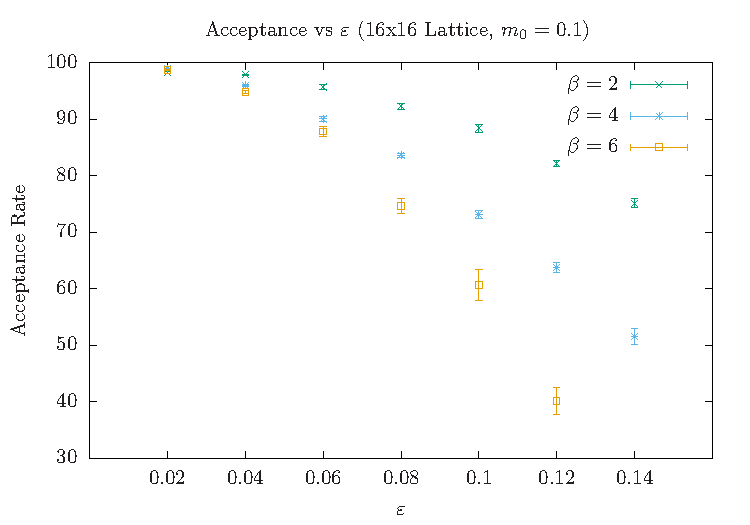
\includegraphics{images/acceps.pdf}
    \caption{Acceptance rate vs $\varepsilon$}
    \label{fig:acc_eps}
\end{figure}
\begin{figure}
    \centering
    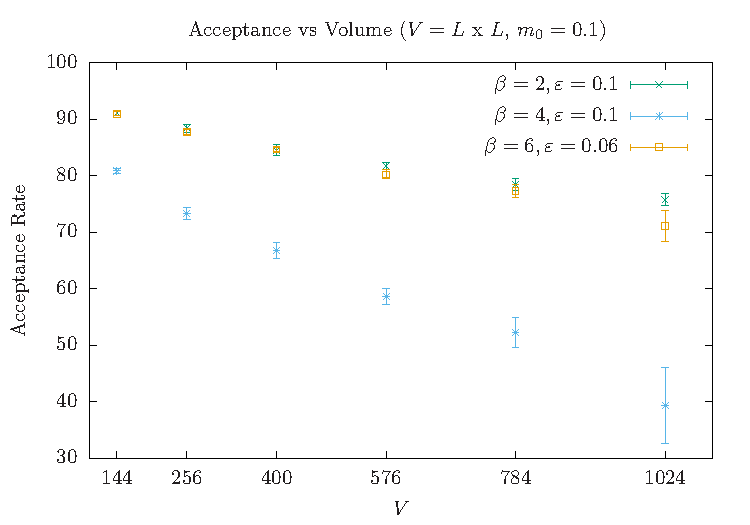
\includegraphics{images/accvol.pdf}
    \caption{Acceptance rate vs $V$}
    \label{fig:acc_vol}
\end{figure}
\\ It is important to work with a sufficiently high acceptance rate, so that one does not waste too much computational resources when taking measurements, hence we need to understand which parameters best fit our requests.
In Figure \ref{fig:acc_eps} we show the dependence of the acceptance rate on the molecular dynamics parameter $\varepsilon$ for a $16 \times 16$ lattice with $m_0 = 0.1$, simulated for different values of the gauge coupling $\beta = 1/g^2$. For small values of $\varepsilon$, the configuration proposed at the end of the trajectory is not that far from the previous one, so it is more likely to be accepted and indeed the acceptance rate is high, independently from the value of $\beta$. As soon as we start to increase the value of $\varepsilon$, the acceptance rate starts decaying quite rapidly: one can clearly see that the acceptance rate falls at a higher pace for smaller values of $\beta.$ 
\\ In Figure \ref{fig:acc_vol} we show the dependence of the acceptance rate on the volume: we simulated square lattices ($L \times L$) with $m_0 = 0.1$ and for different values of the gauge coupling. Notice that for $\beta = 2$ and $4$ we fixed $\varepsilon = 0.1$, while for $\beta = 6$ we embedded a lower value for $\varepsilon$, since simulations with $\varepsilon = 0.1$ produced very low acceptance rates. Coincidentally, in this way we tuned the acceptance rates of the lattices with $\beta = 2$ and $\beta = 6$, and it shows how their dependence on the volume is pretty similar.
\\ Generally, one can conclude that the acceptance rate has a softer dependence on the volume, as it does not decay that rapidly.
Given the above results, we tried to adapt our model parameters in order to always have an acceptance rate of at least $\sim 70\%.$
